\section{Materiales y métodos}
\label{sec:metodos}

\subsection{Protocolo experimental}
\label{sec:protocolo}
\pendiente{Un voluntario (V1), ubicación de los electrodos, registro de 1 min en reposo, actividad física y registro de 3 min posterior.}

\subsection{Sistema de adquisición}
\label{sec:adquisicion}

La cadena de adquisición está formada por tres electrodos descartables, el módulo AD8232 de SparkFun, un Arduino UNO y una interfaz gráfica en Python que corre en la computadora \parencite{tassara_ecg}. El módulo amplifica y filtra la señal en forma analógica. El Arduino la digitaliza con su conversor de 10 bits y la envía por el puerto serie, y la interfaz la grafica en tiempo real y, al terminar, la guarda en un archivo.

\subsubsection{Resolución de la placa AD8232}
\label{sec:resolucion}
% Responde: ítem 3a

El AD8232 es un front-end analógico. Integra un amplificador de instrumentación, un amplificador operacional, el amplificador de pierna derecha activa y la detección de electrodo suelto, pero no tiene conversor analógico-digital \parencite{analog_ad8232}. Por eso no tiene una resolución en bits: su desempeño se describe por la ganancia, el ancho de banda y el ruido. El amplificador de instrumentación tiene ganancia fija de 100 y un rechazo de modo común de al menos \SI{80}{\decibel} entre continua y \SI{60}{\hertz}. Tolera potenciales de contacto de hasta \SI{\pm300}{\milli\volt} y su ruido referido a la entrada es de \SI{14}{\micro\volt} pico a pico entre \SI{0.5}{\hertz} y \SI{40}{\hertz}. Ese ruido es el límite de lo que la placa puede distinguir en la señal.

En el módulo de SparkFun, la etapa de salida tiene ganancia 11, por lo que la ganancia total es 1100. Esa etapa forma además un pasabajos de dos polos, y la red de bloqueo de continua del amplificador de instrumentación, un pasaaltos también de dos polos. Simulamos la respuesta en frecuencia con los valores de los componentes del esquemático \parencite{sparkfun_hw} y obtuvimos una banda de paso a \SI{-3}{\decibel} de aproximadamente \SI{0.4}{\hertz} a \SI{44}{\hertz}, que coincide con la configuración de monitor cardíaco de la hoja de datos (pasaaltos en \SI{0.5}{\hertz} y pasabajos en \SI{40}{\hertz}). La placa se alimenta con \SI{3.3}{\volt} y referencia su salida a la mitad de esa tensión, \SI{1.65}{\volt}. La salida puede variar entre \SI{0.1}{\volt} y \SI{3.2}{\volt}.

La resolución con la que efectivamente queda registrada la señal la fija la digitalización. El conversor del Arduino UNO es de 10 bits y toma como referencia la alimentación de \SI{5}{\volt}, de modo que un paso de cuantización vale $\SI{5}{\volt}/1024 \approx \SI{4.9}{\milli\volt}$. Como la salida del módulo solo ocupa el rango de \SI{0.1}{\volt} a \SI{3.2}{\volt}, se usan unos 635 de los 1024 niveles posibles, algo más de 9 bits efectivos. Dividido por la ganancia, un paso de cuantización equivale a \SI{4.4}{\micro\volt} en los electrodos.

La interfaz empeora un poco este valor, porque al guardar redondea cada muestra a dos decimales en voltios, es decir, a pasos de \SI{10}{\milli\volt}. La resolución real del archivo es entonces de \SI{10}{\milli\volt} a la salida del módulo, unos \SI{9}{\micro\volt} referidos a la entrada. Ese valor es del mismo orden que el ruido propio del amplificador y unas cien veces menor que la amplitud de un complejo QRS, que ronda \SI{1}{\milli\volt}.

\subsubsection{Formato del registro}
\label{sec:formato}
% Responde: ítem 1 (primera parte)

La interfaz guarda cada registro en un archivo de texto con valores separados por comas (CSV) \parencite{tassara_ecg}. El archivo tiene una sola columna: la primera fila es el encabezado \texttt{Sample} y cada fila siguiente es una muestra. Cada valor es la tensión a la salida del módulo en voltios, que la interfaz calcula a partir de la cuenta del conversor $n$ como $V = 5\,n/1023$ y redondea a dos decimales. Los valores quedan entre \SI{0.10}{\volt} y \SI{3.20}{\volt}, centrados cerca de \SI{1.65}{\volt}.

El archivo no incluye columna de tiempo, frecuencia de muestreo, unidades, ganancia ni identificación del sujeto o de la derivación. Además, la conversión a voltios supone que la referencia del conversor es exactamente \SI{5}{\volt}, cuando en realidad depende de la tensión que entrega el puerto USB. Esto puede introducir un error de algunos puntos porcentuales en la amplitud absoluta, que no afecta ni la detección de latidos ni los intervalos RR.

\subsubsection{Frecuencia de muestreo}
\label{sec:fs}
% Responde: ítem 2

Como el archivo no guarda una base de tiempo, la frecuencia de muestreo no se puede leer del registro y hay que deducirla del firmware del Arduino y de la cantidad de muestras de cada registro. El programa configura el Timer1 del microcontrolador en modo CTC, con el reloj de \SI{16}{\mega\hertz} y un divisor $N = 64$, y en cada interrupción del timer lee una muestra del conversor. La frecuencia de las interrupciones la fija el registro de comparación \texttt{OCR1A}:
\begin{equation}
  f_s = \frac{f_\text{clk}}{N\,(1 + \texttt{OCR1A})} = \frac{\SI{16}{\mega\hertz}}{64 \cdot 500} = \SI{500}{\hertz},
  \label{eq:fs}
\end{equation}
es decir, una muestra cada \SI{2}{\milli\second}. El firmware publicado trae \texttt{OCR1A} en 999, que da \SI{250}{\hertz}, y, como alternativa comentada, en 499, que da \SI{500}{\hertz} \parencite{tassara_ecg}. Los registros muestran que se usó la segunda. El de reposo tiene \num{28800} muestras y el post ejercicio, \num{86600}: a \SI{250}{\hertz} equivaldrían a \SI{115}{\second} y \SI{346}{\second}, casi el doble de lo que duró cada registro según el protocolo (1 y \SI{3}{\minute}). A \SI{500}{\hertz} equivalen a \SI{57.6}{\second} y \SI{173.2}{\second}.

Las muestras se acumulan en paquetes de 100, equivalentes a \SI{0.2}{\second} de señal, que se envían en binario, con dos bytes por muestra, cada vez que la interfaz los pide. Esta transmisión limita el muestreo. El puerto serie funciona a 9600 baudios; con 10 bits por byte, transmite 960 bytes por segundo, es decir, 480 muestras por segundo, menos que las 500 que toma el timer. Mientras se envía un paquete, el Arduino llena el siguiente, pero el envío tarda \SI{0.208}{\second} y el paquete se completa en \SI{0.2}{\second}. Mientras espera el próximo pedido, el firmware deja de guardar muestras durante unos \SI{8}{\milli\second}. Cada paquete es continuo, pero entre un paquete y el siguiente se pierden unas 4 muestras. Lo comprobamos en los registros: el salto entre muestras consecutivas es, en promedio, unas 4,5 veces mayor en el borde entre paquetes que en cualquier otra posición, algo que no ocurre si se agrupan las muestras en bloques de otro tamaño. Esto explica también la cantidad de muestras de cada registro: \num{28800} en \SI{1}{\minute} y \num{86600} en \SI{3}{\minute} dan una tasa media de 480 muestras por segundo, justo lo que permite el enlace.

En el análisis usamos $f_s = \SI{500}{\hertz}$, que es la separación real entre muestras dentro de cada paquete. Al no tener en cuenta los huecos, el eje de tiempo queda comprimido un \SI{4}{\percent}: los intervalos RR resultan un \SI{4}{\percent} más cortos, y la frecuencia cardíaca y las frecuencias del espectro, un \SI{4}{\percent} más altas. Este error es sistemático y el mismo en todos los registros, por lo que no cambia las comparaciones entre condiciones. Además, como la cantidad de huecos dentro de un intervalo RR varía de un latido a otro, cada intervalo tiene una incertidumbre adicional de hasta \SI{8}{\milli\second}.

El código de la interfaz define internamente una frecuencia de \SI{100}{\hertz} (variable \texttt{sampling\_rate}), que usa solo para la estimación de frecuencia cardíaca que muestra en pantalla. Ese valor no coincide con el firmware, por lo que esa estimación no es confiable.

La frecuencia de muestreo es adecuada para este trabajo. La frecuencia de Nyquist es \SI{250}{\hertz}. A esa frecuencia el pasabajos del módulo atenúa unos \SI{30}{\decibel}, y el ECG tiene muy poca energía por encima de \SI{40}{\hertz}, de modo que el solapamiento espectral es despreciable. Para el análisis de variabilidad, \SI{500}{\hertz} permite ubicar cada pico R con una resolución de \SI{2}{\milli\second}. \textcite{kwon2018} compararon distintas frecuencias de muestreo y encontraron que ya con \SI{250}{\hertz} los índices de variabilidad, tanto temporales como espectrales, tienen excelente concordancia con los obtenidos a \SI{500}{\hertz}.

\subsection{Acondicionamiento de la señal}
\label{sec:met-acondicionamiento}
% Responde: ítem 4

La señal necesita acondicionamiento antes del análisis. El módulo ya la filtra aproximadamente entre \SI{0.5}{\hertz} y \SI{40}{\hertz}, pero el registro, tal como lo guarda la interfaz, contiene componentes que no provienen del corazón sino de la propia cadena de adquisición. Dejamos de lado los artefactos fisiológicos (respiración, actividad muscular y movimiento), que la consigna excluye. Los ruidos y defectos asociados al registro son los siguientes:

\begin{itemize}
  \item \textbf{Nivel de continua.} La salida está referida a \SI{1.65}{\volt}, así que todo el registro está montado sobre ese valor. No es un ruido en sentido estricto, pero hay que quitarlo para trabajar con una señal centrada en cero.
  \item \textbf{Deriva de la línea de base.} La interfaz entre el electrodo y la piel genera un potencial de media celda que cambia lentamente con el secado del gel, la presión y la temperatura. El pasaaltos del módulo atenúa estas variaciones pero no las elimina, y además tarda en estabilizarse después de colocar los electrodos o de una saturación. Se ve como una ondulación lenta del nivel de base, por debajo de \SI{1}{\hertz}.
  \item \textbf{Interferencia de línea.} La red eléctrica (\SI{50}{\hertz} en Argentina) se acopla capacitivamente al cuerpo y a los cables, y también puede entrar por la computadora, que alimenta al Arduino por USB. El rechazo de modo común y la pierna derecha activa la reducen, pero el pasabajos del módulo, con corte en \SI{40}{\hertz}, la atenúa apenas unos \SI{4}{\decibel}. Cuando está presente, se ve como una oscilación rápida superpuesta al trazado y como un pico en \SI{50}{\hertz} en el espectro. En nuestros registros, sin embargo, el espectro no muestra ese pico: la densidad espectral en \SI{50}{\hertz} es igual o menor que la de las frecuencias vecinas (figura~\ref{fig:acond_espectro_crudo}).
  \item \textbf{Ruido de cuantización.} Por el redondeo a \SI{10}{\milli\volt} que hace la interfaz, la señal avanza en escalones visibles en los tramos de baja amplitud, como las ondas P y T y el segmento isoeléctrico. Es pequeño frente al QRS y no afecta la detección de latidos, pero la información perdida no se puede recuperar.
  \item \textbf{Saturación.} La salida solo puede alejarse unos \SI{1.55}{\volt} de la referencia hacia cada lado, lo que con ganancia 1100 equivale a unos \SI{1.4}{\milli\volt} en la entrada. Una onda R grande o un salto brusco del potencial de contacto llevan la salida al extremo y la recortan. En el registro post ejercicio la salida llega a \SI{0}{\volt} y a \SI{3.3}{\volt}: muchas ondas R quedan recortadas en unas pocas muestras y la deriva lleva la línea de base al mínimo en varios tramos de hasta \SI{0.35}{\second} (figura~\ref{fig:acond_detalles}b). El registro de reposo no satura. El firmware tampoco lee las salidas de detección de electrodo suelto (LO+ y LO$-$), aunque estén cableadas, de modo que un electrodo despegado no queda marcado en el archivo: solo se reconoce como un tramo plano en \SI{0.1}{\volt} o en \SI{3.2}{\volt}.
  \item \textbf{Discontinuidad al inicio.} Antes de que se presione \textit{Comenzar grabación}, el Arduino llena su primer paquete de 100 muestras y queda esperando el pedido de la interfaz. Ese paquete, tomado en un momento anterior, es el primero que se guarda, por lo que las primeras \SI{0.2}{\second} del archivo no son continuas con el resto. Si se graba más de una vez sin desconectar, pueden acumularse dos paquetes viejos. En el registro post ejercicio se ven \SI{0.1}{\second} saturados al comienzo y saltos a los \SI{0.1}{\second} y a los \SI{0.3}{\second}, separados justamente por un paquete (figura~\ref{fig:acond_detalles}a).
\end{itemize}

Hay también una exigencia propia del análisis de variabilidad. El resultado final son los instantes de los latidos, así que el filtrado no debe desplazar la señal en el tiempo. Por eso los filtros deben aplicarse sin desfasaje.

El acondicionamiento debe, entonces, descartar el primer segundo de cada registro, quitar el nivel de continua y la deriva de la línea de base con un pasaaltos de corte bajo y detectar los tramos saturados para excluirlos. La interferencia de \SI{50}{\hertz} no aparece en los registros, por lo que no se aplicó un filtro específico para ella. El ruido de cuantización y el ruido electrónico del amplificador quedan por debajo de lo que afecta a la detección y no requieren un tratamiento específico. El algoritmo de Pan-Tompkins incluye su propio pasabanda, pero el acondicionamiento previo sigue siendo necesario para inspeccionar la morfología, graficar los registros y evitar que los umbrales del detector dependan de la deriva o de la interferencia.

La figura~\ref{fig:acond_crudo} muestra los registros completos tal como los guarda la interfaz. Los dos están montados sobre \SI{1.65}{\volt}. En reposo la línea de base es estable y la señal no satura; en el registro post ejercicio la deriva supera \SI{1}{\volt} y la señal recorre todo el rango de salida. En el espectro (figura~\ref{fig:acond_espectro_crudo}) esa deriva aparece como potencia concentrada por debajo de \SI{0.5}{\hertz}, unas cien veces mayor en el registro post ejercicio que en el de reposo. La figura~\ref{fig:acond_detalles} muestra en detalle la discontinuidad del inicio, un tramo saturado y los escalones de cuantización.

\begin{figure}[htbp]
  \centering
  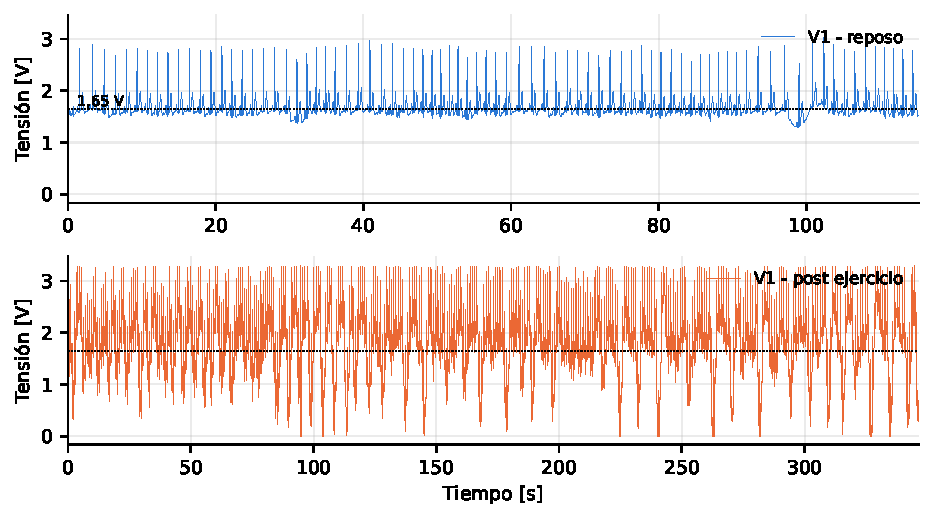
\includegraphics[width=\textwidth]{acond_crudo_completo}
  \caption{Registros crudos de V1 en reposo y post ejercicio. La línea punteada marca la referencia de \SI{1.65}{\volt}.}
  \label{fig:acond_crudo}
\end{figure}

\begin{figure}[htbp]
  \centering
  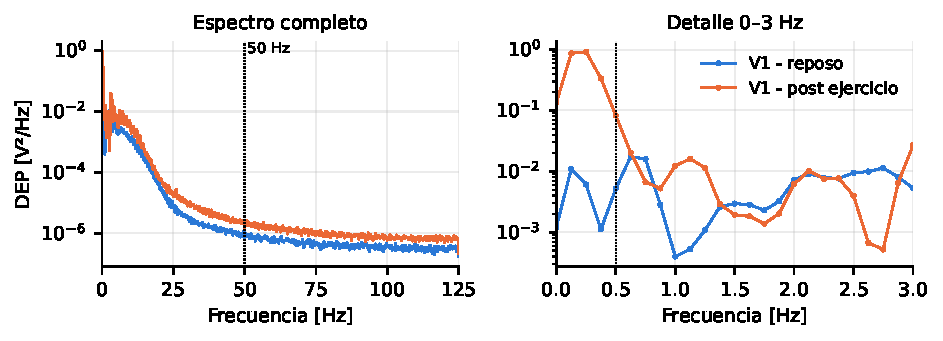
\includegraphics[width=\textwidth]{acond_espectro_crudo}
  \caption{Densidad espectral de potencia de los registros crudos (Welch, ventanas de \SI{8}{\second}). Izquierda: espectro completo; la línea punteada marca \SI{50}{\hertz}. Derecha: detalle de 0 a \SI{3}{\hertz}; la línea punteada marca el corte del pasaaltos, \SI{0.5}{\hertz}.}
  \label{fig:acond_espectro_crudo}
\end{figure}

\begin{figure}[htbp]
  \centering
  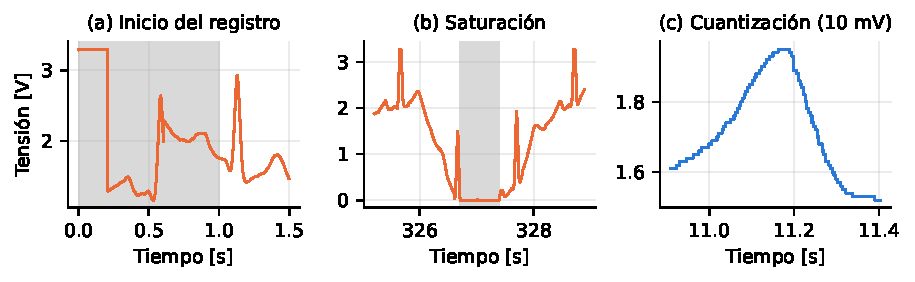
\includegraphics[width=\textwidth]{acond_detalles}
  \caption{Defectos del registro. (a) Primer segundo del registro post ejercicio, que se descarta (sombreado). (b) Tramo saturado en \SI{0}{\volt} del registro post ejercicio (sombreado). (c) Onda T del registro en reposo, con los escalones de \SI{10}{\milli\volt} del redondeo de la interfaz.}
  \label{fig:acond_detalles}
\end{figure}

\paragraph{Etapas implementadas (ítem 5).}
El acondicionamiento se aplica en el orden de la tabla~\ref{tab:acond}. Primero se reemplazan por una recta los tramos saturados de más de \SI{0.1}{\second}: dentro de ellos la señal real es desconocida, y la meseta, con sus escalones de entrada y salida, haría oscilar al pasaaltos. Las puntas de onda R recortadas duran unas pocas muestras y no se tocan, para no mover el pico. Después se resta la mediana del registro, que es menos sensible que la media a los tramos saturados, y se aplica un pasaaltos Butterworth con corte en \SI{0.5}{\hertz}. El corte queda por debajo de la frecuencia cardíaca más baja esperable y deja pasar el complejo QRS completo, cuya energía se concentra entre 5 y \SI{15}{\hertz} \parencite{pan1985}.

El pasaaltos se aplica hacia adelante y hacia atrás (\texttt{sosfiltfilt} de SciPy). La respuesta resultante tiene fase nula y módulo igual al cuadrado del filtro original, por lo que la señal acondicionada tiene la misma cantidad de muestras que la cruda y los picos no se desplazan. Lo comprobamos sobre los picos de los dos registros: el corrimiento mediano es nulo y el máximo, de 5 muestras, aparece en una punta recortada, donde la posición del máximo dentro de la meseta no está definida.

El primer segundo y los tramos saturados largos, con un margen de \SI{0.2}{\second} a cada lado, no se borran de la señal, para conservar su longitud, sino que se marcan en una máscara de muestras válidas (función \texttt{mascara\_valida}). Los latidos que caen en esas zonas se descartan al construir el tacograma. La máscara excluye el \SI{1.7}{\percent} del registro de reposo y el \SI{2.7}{\percent} del registro post ejercicio. No se aplicó notch ni pasabajos: no hay interferencia de red, y el módulo ya limita la banda a unos \SI{40}{\hertz}.

\begin{table}[htbp]
  \centering
  \caption{Etapas de acondicionamiento y sus parámetros.}
  \label{tab:acond}
  \begin{tabular}{@{}p{3.8cm}p{3.6cm}p{7.6cm}@{}}
    \toprule
    Etapa & Defecto que corrige & Parámetros \\
    \midrule
    Interpolación de saturaciones & Saturación & Tramos $\geq \SI{0.1}{\second}$ a menos del \SI{1}{\percent} del rango de los extremos \\
    Resta de la mediana & Nivel de continua & --- \\
    Pasaaltos Butterworth & Deriva de la línea de base & $f_c = \SI{0.5}{\hertz}$, orden 2, fase cero (orden 4 efectivo) \\
    Máscara de muestras válidas & Inicio y saturación & Primer \SI{1}{\second}; tramos saturados $\pm\SI{0.2}{\second}$ \\
    \bottomrule
  \end{tabular}
\end{table}

\subsection{Detección de latidos: algoritmo de Pan-Tompkins}
\label{sec:met-pantompkins}
% Responde: ítem 6 (método)
\pendiente{Etapas del algoritmo y parámetros usados.}

\subsection{Tacograma}
\label{sec:met-tacograma}
\pendiente{Construcción de la serie RR y métricas reportadas.}

\subsection{Periodograma de Lomb}
\label{sec:met-lomb}
% Responde: ítem 7 (método)

El tacograma no es una señal muestreada en forma uniforme: cada valor RR queda ubicado en el instante del latido que cierra el intervalo, y la separación entre muestras es justamente el propio RR, que varía. Además le faltan los latidos que se descartan en las zonas inválidas del registro (sección~\ref{sec:met-acondicionamiento}). La transformada de Fourier discreta supone muestras equiespaciadas, por lo que la alternativa habitual es interpolar el tacograma y remuestrearlo a una frecuencia fija. La interpolación, sin embargo, actúa como un pasabajos que atenúa las componentes rápidas y obliga a inventar valores en los huecos. El periodograma de Lomb evita ese paso: para cada frecuencia ajusta por cuadrados mínimos un coseno y un seno evaluados en los instantes reales de las muestras \parencite{lomb1976}. \textcite{laguna1998} mostraron que es adecuado para señales de frecuencia cardíaca y que tolera la falta de latidos sin necesidad de rellenarlos.

Para una serie $x_n$ de media nula, tomada en los instantes $t_n$, la potencia en la frecuencia angular $\omega = 2\pi f$ es
\begin{equation}
  P(\omega) = \frac{1}{2}\left[
    \frac{\left(\sum_n x_n \cos\omega(t_n-\tau)\right)^2}{\sum_n \cos^2\omega(t_n-\tau)} +
    \frac{\left(\sum_n x_n \sin\omega(t_n-\tau)\right)^2}{\sum_n \sin^2\omega(t_n-\tau)}
  \right],
  \qquad
  \tan(2\omega\tau) = \frac{\sum_n \sin 2\omega t_n}{\sum_n \cos 2\omega t_n},
  \label{eq:lomb}
\end{equation}
donde el corrimiento $\tau$ hace que los ajustes del seno y del coseno sean independientes. Si las muestras son equiespaciadas, $P$ coincide con el periodograma clásico.

\paragraph{Tratamiento previo del tacograma.}
Antes de calcular el periodograma se aplican dos pasos:
\begin{itemize}
  \item \textbf{Descarte de intervalos atípicos.} Un latido no detectado duplica el RR y una detección falsa lo parte en dos. Ambos errores agregan potencia de banda ancha que no es fisiológica. Se descarta cada RR que se aparta más de un \SI{30}{\percent} de la mediana de los 11 intervalos centrados en él. Con un umbral del \SI{20}{\percent} se descartaban dos intervalos reales del registro de reposo, ubicados en las crestas de una oscilación lenta. Como Lomb no necesita muestras equiespaciadas, los intervalos descartados simplemente se quitan, sin interpolar.
  \item \textbf{Quitar la tendencia.} Se resta un polinomio de grado 2 en función del tiempo, ajustado por cuadrados mínimos. Esto quita la media, que Lomb necesita nula, y la tendencia lenta de la recuperación posterior al ejercicio, durante la cual el RR aumenta en forma sostenida. Sin este paso, la tendencia concentra potencia en las frecuencias más bajas y, por las fugas espectrales, contamina la banda LF. Un polinomio de grado 2 sobre registros de 1 a 3 minutos solo sigue variaciones mucho más lentas que \SI{0.04}{\hertz}, de modo que no afecta las bandas analizadas.
\end{itemize}

\paragraph{Frecuencias evaluadas y normalización.}
La resolución en frecuencia está dada por la duración $T$ del tacograma, $1/T$. Se evalúa una grilla cuatro veces más fina, de $1/(4T)$ a \SI{0.5}{\hertz} con paso $1/(4T)$, para ubicar mejor los picos, aunque esto no agrega resolución. El límite de \SI{0.5}{\hertz} cubre la banda HF con margen y queda por debajo de la mitad de la frecuencia media de latidos en todos los registros (más de \SI{0.7}{\hertz} a \SI{84}{lpm}). La potencia se expresa como densidad espectral unilateral, $p(f) = 2P/\bar f_s$, donde $\bar f_s = N/T$ es la cantidad media de latidos por segundo. Con esta escala, el área bajo $p$ es la varianza del tacograma (teorema de Parseval), y la potencia de cada banda se obtiene integrando $p$ en ese rango, en \si{\milli\second\squared}.

\paragraph{Bandas e índices.}
Se usan las bandas de la \textcite{taskforce1996} para registros cortos: LF (baja frecuencia), de \SI{0.04}{\hertz} a \SI{0.15}{\hertz}, y HF (alta frecuencia), de \SI{0.15}{\hertz} a \SI{0.4}{\hertz}. La potencia HF refleja principalmente la modulación vagal ligada a la respiración (arritmia sinusal respiratoria), y el pico dentro de esa banda estima la frecuencia respiratoria. La potencia LF recibe aportes de ambas ramas del sistema autónomo y del barorreflejo. La banda de muy baja frecuencia (VLF, por debajo de \SI{0.04}{\hertz}) no se analiza porque no puede estimarse en registros de menos de \SI{5}{\minute}. Para cada registro se informan la potencia en LF y en HF, el cociente LF/HF y las unidades normalizadas, $\mathrm{LF_{nu}} = \mathrm{LF}/(\mathrm{LF}+\mathrm{HF})$ y $\mathrm{HF_{nu}} = \mathrm{HF}/(\mathrm{LF}+\mathrm{HF})$, que comparan la distribución de la potencia entre las dos bandas sin depender de su valor absoluto \parencite{taskforce1996}.

La \textcite{taskforce1996} recomienda registros de al menos \SI{1}{\minute} para estimar HF y de al menos \SI{2}{\minute} para LF. El registro de reposo, de unos \SI{55}{\second} útiles, alcanza para HF, pero su estimación de LF es solo orientativa. El registro post ejercicio no es estacionario, porque la frecuencia cardíaca baja durante toda la recuperación. Por eso, además de analizarlo completo, se lo dividió en ventanas consecutivas de \SI{1}{\minute}, cada una con su propio tratamiento previo y su propia grilla.

\paragraph{Implementación y validación.}
Todo el procedimiento está en el módulo \texttt{periodograma\_lomb.py}, que implementa la ecuación~\eqref{eq:lomb} con NumPy. Se lo validó con un tacograma sintético de \SI{180}{\second} a \SI{70}{lpm}, cuyo RR oscila un \SI{5}{\percent} a \SI{0.2}{\hertz}. El pico del periodograma quedó en \SI{0.200}{\hertz} y el área bajo la curva coincidió con la varianza de la serie con un error del \SI{0.5}{\percent}. El resultado también coincidió, salvo errores de redondeo, con la función \texttt{lombscargle} de SciPy.